% !TEX root = template.tex

\section{Results}
\label{sec:results}

In this section we will evaluate the performance of our new models in terms of accuracy with respect to the number of parameters that characterize each model. We will also compare our findings with previous state-of-the-art results.

\begin{figure}[htbp]
\centerline{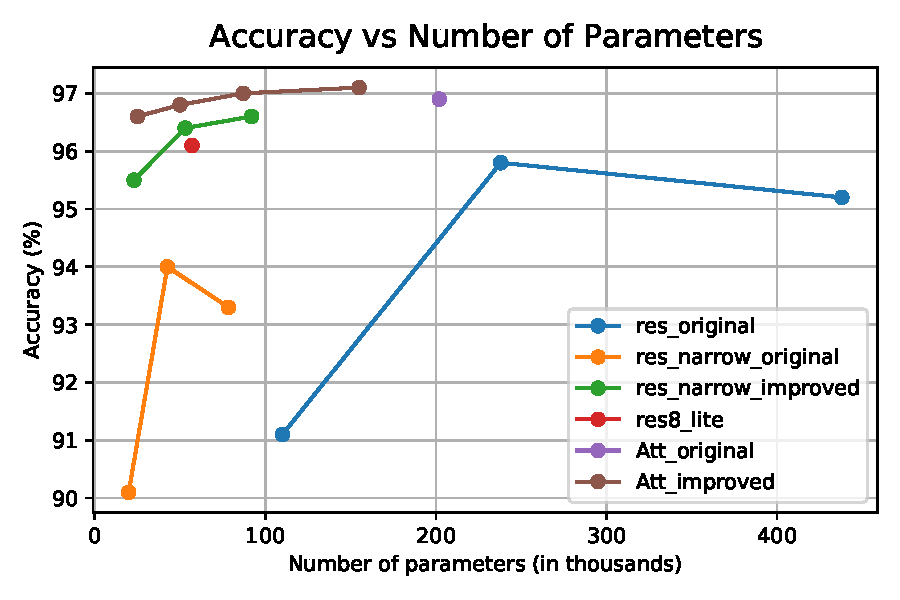
\includegraphics[scale=.6]{acc_vs_par.pdf}}
\caption{Comparison of the accuracy and number of parameters between ours and previous models}
\label{avp}
\end{figure}

In Figure \ref{avp} we can see a comparison between our new models and the most promising models in the literature. The models we presented are refered to Att_improved in brown, res_narrow_improved in green and res8_lite in red.
It is clear that our new models bring a noticeable improvement: our enhanced recurrent neural network models based on the attention obtain similar accuracy results as in [1], while having only a fraction (up to 8 times less) of the parameters. The models Att87K and Att155K even slightly surpass the highest accuracy obtained up to now, that was 96.9\% in [1]. In fact, our models obtained respectively 97\% and 97.18\% while having fewer parameters. 
Our res-net models can achieve at least 2\% higher accuracy than the models presented in [2]. However in this case it is worth noting that in [2] they used an older version of the dataset, and different feature extraction (MFCCs as opposed to Mel-Spectrogram). Overall from our tests it seems that our improved implementation of the attention-based recurrent neural networks provides better models: they obtain high accuracy even with limited amounts of parameters. However even our res-net models obtain satisfying levels of accuracy, and can provide a good alternative.

%\begin{figure*}[!htb]
%    \begin{minipage}[t]{.5\textwidth}
%        \centering
%        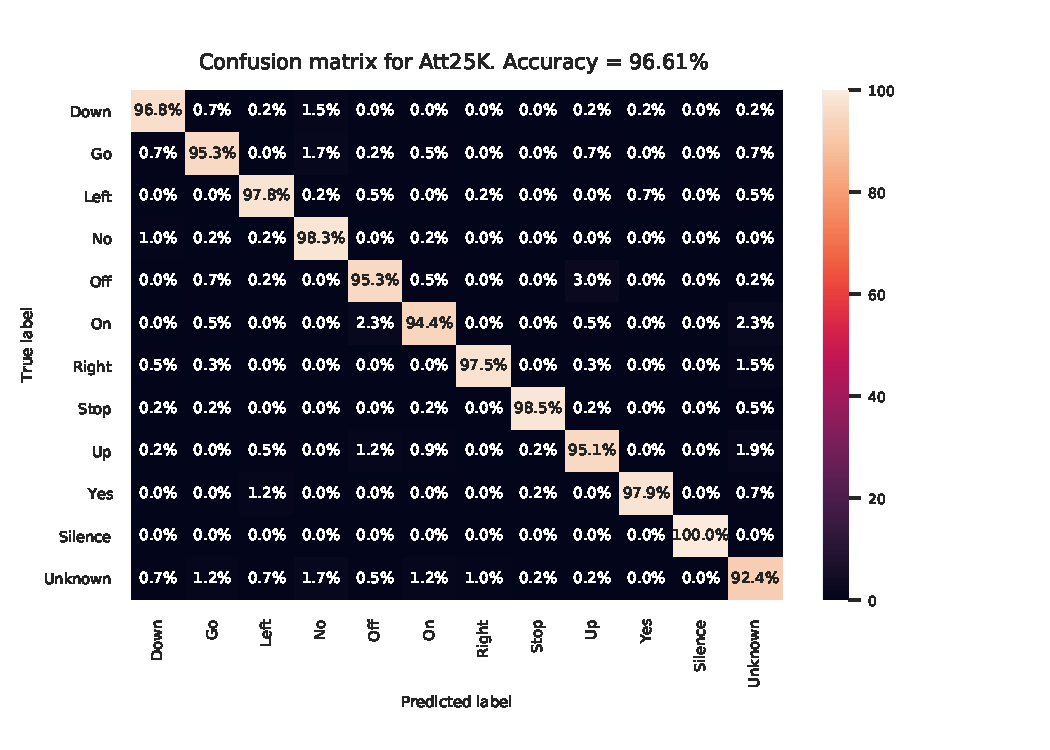
\includegraphics[width=1.1\textwidth]{conf_att.pdf}
%        \subcaption{Image 1.}\label{fig:1}
%    \end{minipage}
%    \hfill
%    \begin{minipage}[t]{.5\textwidth}
%        \centering
%        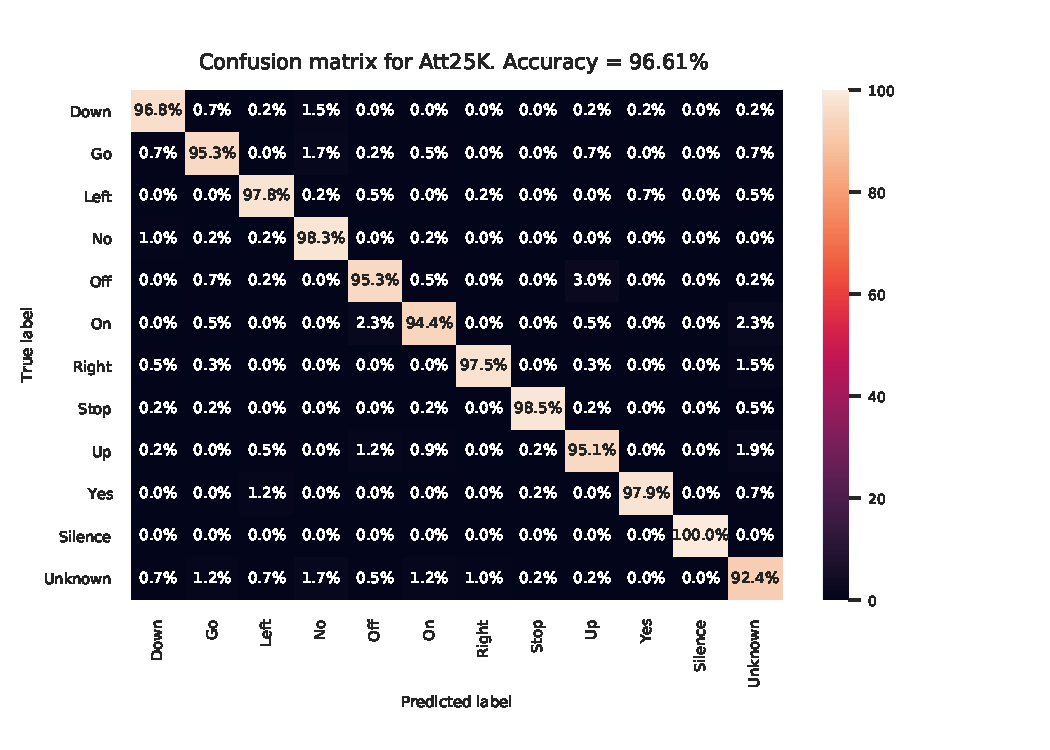
\includegraphics[width=1.1\textwidth]{conf_att.pdf}
%        \subcaption{Image 2.}\label{fig:2}
%    \end{minipage}  
%    \label{fig:1-2}
%    \caption{Title.}
%\end{figure*}

\begin{figure}[htbp]
\centerline{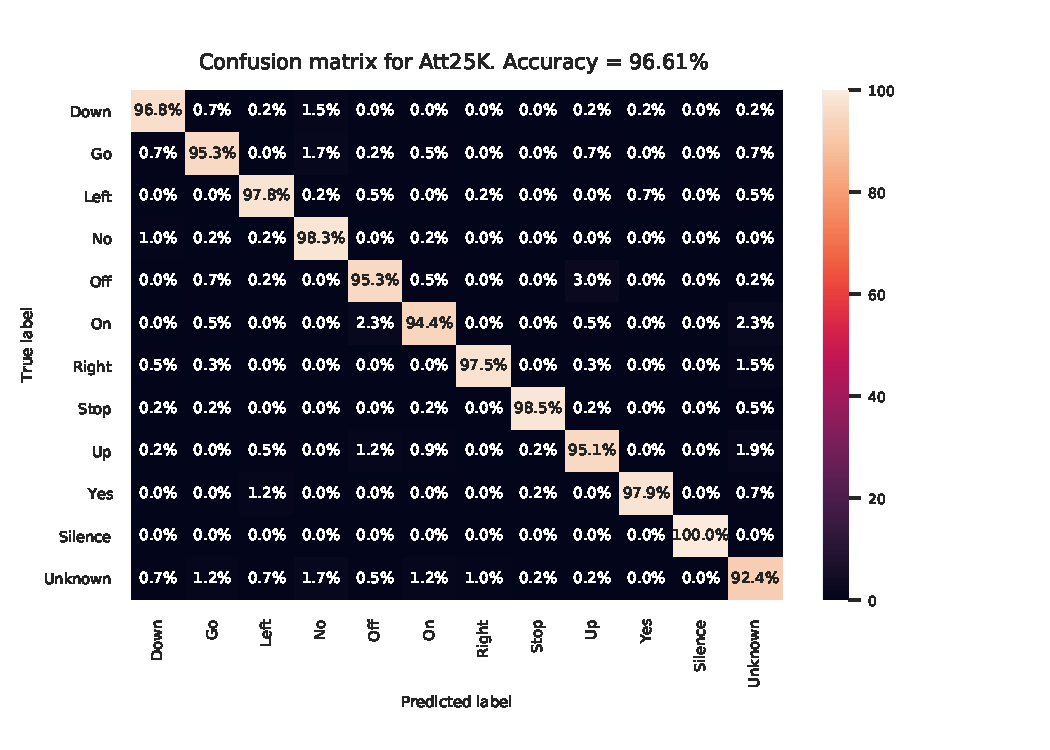
\includegraphics[scale=.5]{conf_att.pdf}}
\caption{Att25K confusion matrix}
\label{conf_att}
\end{figure}

\begin{figure}[htbp]
\centerline{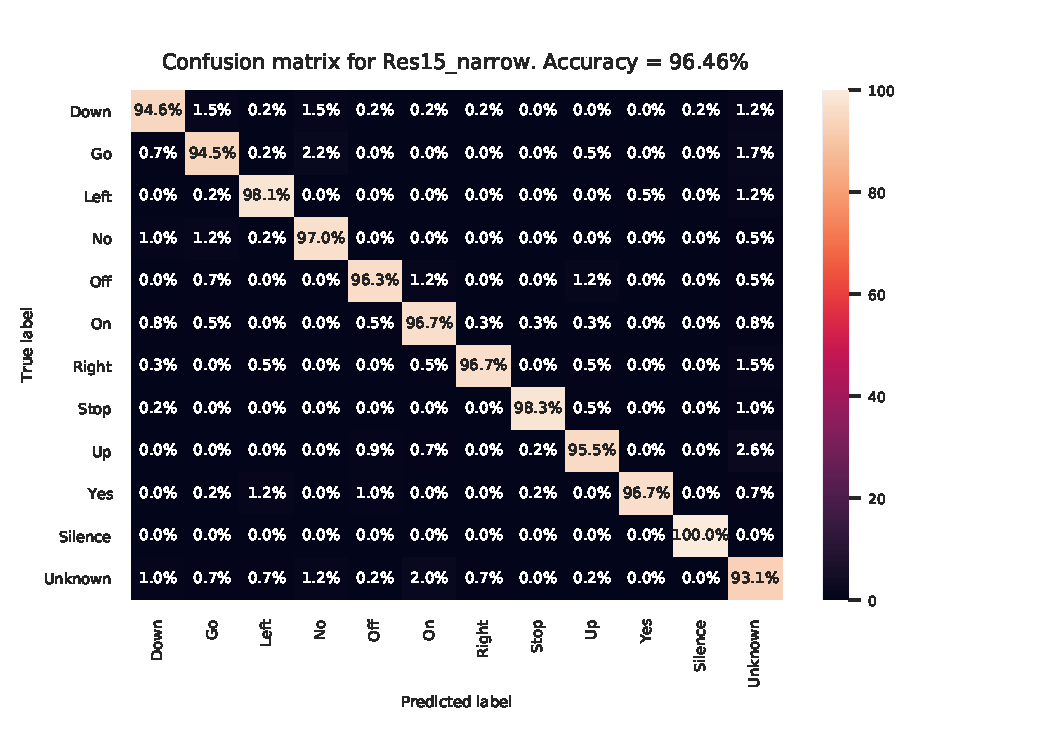
\includegraphics[scale=.5]{conf_res.pdf}}
\caption{Res15_narrow confusion matrix.}
\label{conf_res}
\end{figure}


In Figures \ref{conf_att} and \ref{conf_res} we provide the confusion matrix of our most interesting models, that are Att25K and Res15narrow. Even if it doesn't offer the best accuracy, Att25K is still reasonably accurate (96.6\%) and it only needs a small number of parameters.
Res15narrow represents a good tradeoff, for what concerns the residual-based models, between the number of parameters and accuracy, even if it has more than double the parameters of Att25K.
From both the confusion matrices we can notice that the hardest class to manage is the "Unknown" class.
For that class the accuracy is, respectively, 92.4\% and 93\%, which is low compared to the other classes. We noticed that sometimes unknown samples are interpreted as actual commands, and at the same time some commands are not recognized as such and are classified as unknown words. Another problematic pair of classes that are sometimes misclassified with each other are "on" and "off". For the opposite meaning that these two commands have, this can actually be a relevant problem in a final application and would need further addressing.


\begin{figure}[htbp]
\centerline{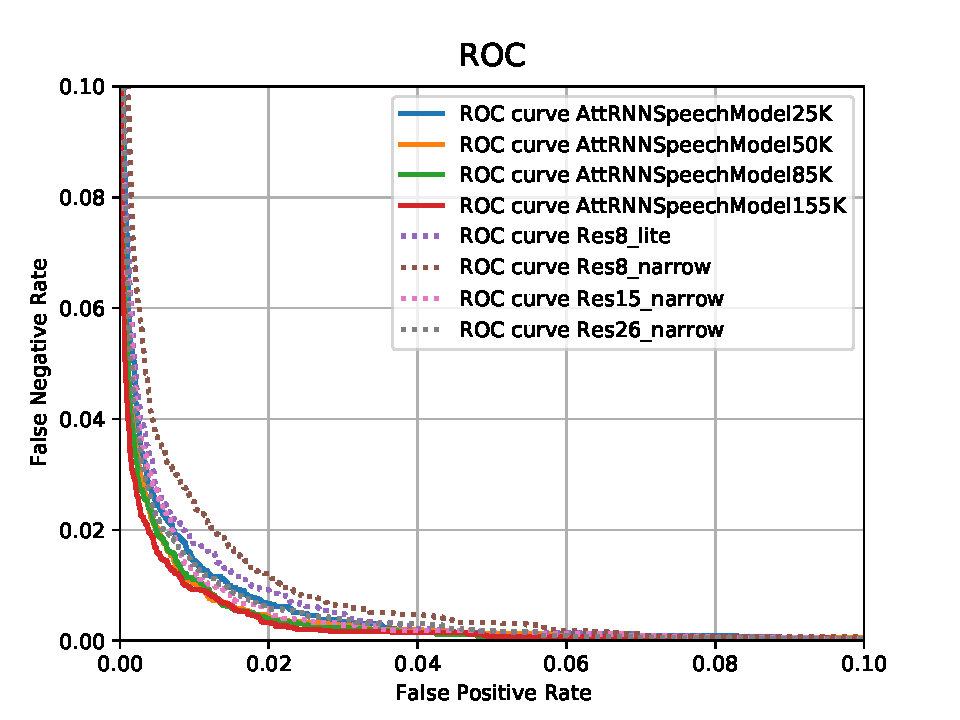
\includegraphics[scale=.5]{ROC.pdf}}
\caption{ROC curves for the different models.}
\label{roc}
\end{figure}

In order to further compare our new models, we show the receiver operating characteristic (ROC) curves. In Figure \ref{roc} the x-axis represents the false-positive rate, while the y-axis shows the false-negative rate, and each point of the curve is computed by considering a different threshold. Every curve corresponds to a single model and it is computed by micro averaging all the curves for each class compared with all the other classes. The models that have a smaller area under the corresponding curve are better. We can notice that the curves of our models are almost all comparable.
